\documentclass[11pt]{article}

% --- Geometry & typography ------------------------------------------------
\usepackage[letterpaper,margin=1in]{geometry}
\usepackage[T1]{fontenc}
\usepackage[utf8]{inputenc}
\usepackage[protrusion=true,expansion=false]{microtype}
\usepackage{setspace}
\setstretch{1.12}

% --- Math & algorithms ----------------------------------------------------
\usepackage{amsmath, amssymb, amsfonts, amsthm}
\usepackage{mathtools}
\usepackage{bm}
\usepackage{algorithm}
\usepackage{algpseudocode}

% --- Tables and figures ---------------------------------------------------
\usepackage{booktabs}
\usepackage{array}
\usepackage{tabularx}
\usepackage{longtable}
\usepackage{makecell}
\usepackage{graphicx}
\renewcommand\theadfont{\bfseries\small}

% --- Code listings ---------------------------------------------------------
\usepackage{xcolor}
\definecolor{borderGray}{RGB}{100, 116, 139}
\definecolor{jsonKey}{RGB}{30, 64, 175}
\definecolor{jsonStr}{RGB}{4, 120, 87}
\definecolor{jsonNum}{RGB}{180, 83, 9}
\definecolor{jsonCmt}{RGB}{107, 114, 128}
\usepackage{listings}
\lstdefinelanguage{jsonpretty}{
  basicstyle=\ttfamily\footnotesize,
  numbers=none,
  showstringspaces=false,
  breaklines=true,
  frame=single,
  rulecolor=\color{borderGray},
  framesep=4pt,
  xleftmargin=8pt,
  xrightmargin=8pt,
  literate=
    *{0}{{{\color{jsonNum}0}}}{1}
     {1}{{{\color{jsonNum}1}}}{1}
     {2}{{{\color{jsonNum}2}}}{1}
     {3}{{{\color{jsonNum}3}}}{1}
     {4}{{{\color{jsonNum}4}}}{1}
     {5}{{{\color{jsonNum}5}}}{1}
     {6}{{{\color{jsonNum}6}}}{1}
     {7}{{{\color{jsonNum}7}}}{1}
     {8}{{{\color{jsonNum}8}}}{1}
     {9}{{{\color{jsonNum}9}}}{1}
     {:}{{{\color{borderGray}{:}}}}{1}
     {,}{{{\color{borderGray}{,}}}}{1}
     {\{}{{{\color{borderGray}{\{}}}}{1}
     {\}}{{{\color{borderGray}{\}}}}}{1}
     {[}{{{\color{borderGray}{[}}}}{1}
     {]}{{{\color{borderGray}{]}}}}{1},
  morestring=[b]",
  stringstyle=\color{jsonStr},
  commentstyle=\color{jsonCmt}\itshape,
  morecomment=[l]{//}
}

% --- Layout, lists, headers -----------------------------------------------
\usepackage{enumitem}
\setlist{itemsep=2pt, topsep=3pt}
\usepackage{titlesec}
\titleformat{\section}{\normalfont\large\bfseries}{\thesection.}{0.6em}{}
\titleformat{\subsection}{\normalfont\normalsize\bfseries}{\thesubsection}{0.6em}{}
\titlespacing*{\section}{0pt}{14pt}{6pt}
\titlespacing*{\subsection}{0pt}{10pt}{4pt}

\usepackage{fancyhdr}
\pagestyle{fancy}
\fancyhf{}
\renewcommand{\headrulewidth}{0pt}
\fancyfoot[C]{\thepage}
\fancyhead[L]{\footnotesize\itshape Adversarial Intent Telemetry: An Empirical Study}
\fancyhead[R]{\footnotesize\itshape Draft v9.0, July 2026}

\usepackage[hidelinks]{hyperref}
\usepackage{xurl} % allow URLs to break anywhere (fixes overfull reference lines)

% --- Anonymization switch (for double-blind submission, flip to \anonymoustrue)
\newif\ifanonymous
\anonymousfalse

% =====================================================================
\title{\vspace{-1.2cm}\textbf{Adversarial Intent Telemetry:\\An Empirical Study of Behavioral-Signature Detection\\Under Adaptive Perturbation}}
\ifanonymous
\author{Anonymous submission}
\else
\author{Fahrawn Gill\\ \small Advisor, AI Governance \& Cross-Platform Safety \\ \small Alliance to Counter Crime Online (ACCO)}
\fi
\date{Draft v9.0 \textbullet\ July 2026}

% =====================================================================
\begin{document}
\maketitle
\thispagestyle{fancy}

% --- Abstract ------------------------------------------------------------
\begin{abstract}
\noindent Cross-platform safety infrastructure has succeeded at exchanging \emph{content} signatures: perceptual hashes of known abuse imagery interoperate across providers at production scale. A natural next step is to exchange \emph{behavioral} signatures --- structural fingerprints of adversarial conversations, shared before harmful content exists. A prior design document (v8.1, included with this artifact) specified such a scheme: feature manifests extracted from conversations, matched across providers with banded MinHash signatures, backed by a trajectory-level sequence model. This paper treats that design as the object under test and asks a narrow, falsifiable question: does it survive contact with real adversarial data and adaptive perturbation?

The answer is mixed, and the decomposition is the contribution. On the PAN 2012 Sexual Predator Identification corpus, a per-message linear classifier detects grooming conversations well (AUC 0.986; recall 0.95 at FPR $\leq 0.05$). The design's core cross-provider primitive does not: at the recommended banded-MinHash operating point $(b{=}16, r{=}16)$, recall on real conversations is 0.018 at FPR 0.0013, and usable recall (0.92) appears only at FPR 0.99, falsifying the signature primitive's utility on real text at any deployable false-positive rate. The trajectory-level sequence model does not beat the per-message baseline on clean data (F1 lift $-0.023$, bootstrap 95\% CI $[-0.042, -0.002]$). One robustness signal survives stricter testing but changes attribution: across controlled discourse-noise perturbation sweeps (five seeds, three non-zero strengths), the sequence model's AUC degrades less than the per-message baseline's at every strength, the result replicates under an author-disjoint split (heavy-noise AUC drop 0.029 vs.\ 0.058), and paired bootstrap intervals exclude zero against every per-message comparison. Matched controls, however, show that the advantage is not trajectory structure: an order-invariant control that differs from the sequence model only by removing its position weights is at least as robust, and shuffling message order leaves the sequence model essentially unchanged. What survives is that conversation-level averaging is more perturbation-robust than per-message scoring. A false-positive substrate analysis on structurally similar benign PAN conversations did not find elevated false-positive rates relative to random benign controls (0.030 vs.\ 0.055 for the classifier). All findings are bounded by two stated limits: the perturbation results cover two rule-based noise families, not an adaptive adversary, and PAN 2012 is a historical human-grooming corpus, not evidence about 2026 agentic automation. Byzantine-tolerance results are simulations and the reciprocity mechanism is analytical; neither is deployment evidence. The artifact includes claim-consistency checks that verify every headline number in this paper and the repository README against the committed result files.
\end{abstract}

% =====================================================================
\section{Introduction}
\label{sec:intro}

Content-hash exchange is the one piece of cross-platform trust-and-safety infrastructure with an unambiguous production track record. PhotoDNA-class perceptual hashing sustains sub-millisecond matching against ten-million-hash corpora [18]; the Tech Coalition's Lantern program has moved over two million safety signals across sixty member companies [5]; the Video Hash Interoperability Project (VHIP) demonstrated that \emph{approximate}-match signatures interoperate across heterogeneous vendor pipelines [5]. Meanwhile, the same reporting shows the abuse surface moving upstream of content: AI-related signals through Lantern grew seventeen-fold in 2025, and the agentic-security literature documents adaptive prompt-level attacks succeeding against state-of-the-art defenses [1, 2, 4]. It is therefore tempting to extend the content-hash pattern one layer up: extract structural features from a conversation, hash them into a compact signature, and share the signature across providers so that adversarial \emph{behavior} detected at one platform becomes detectable at its peers before content is ever generated.

That temptation should be tested, not assumed. Content hashes work because two copies of the same image are nearly identical objects; the matching problem is re-identification. Behavioral signatures face a different problem: two conversations executing the same adversarial strategy are \emph{different texts}, and the question is whether any fixed structural representation places them close together --- and benign conversations far apart --- reliably enough to match at a false-positive rate a deployment could tolerate. Success at the content layer carries no guarantee at the behavioral layer.

A prior design document (``Decentralized Telemetry for Adversarial AI Intent,'' v8.1, included with this artifact) specified a complete scheme of this kind: canonical feature manifests, banded MinHash signatures for cross-provider matching, a trajectory-level sequence model, trust-decay scheduling for federated aggregation, and a governance mapping. This paper does not announce that design. It evaluates it. The design is the hypothesis; the experiments reported here are the test; and several of the design's load-bearing claims do not survive.

We state the mixed result up front.
\begin{itemize}[leftmargin=1.5em]
\item A strong per-message baseline (LinearSVC over character n-grams) detects grooming conversations in the PAN 2012 corpus at AUC 0.986, with recall 0.95 at FPR 0.05 --- behavioral structure in real adversarial conversations is detectable (Sec.~\ref{sec:rq1}).
\item The design's core cross-provider primitive fails on the same data. Banded MinHash matching at the recommended operating point recalls 1.8\% of real predator conversations at FPR 0.0013; pushing recall to 0.92 requires accepting FPR 0.99. There is no usable operating point on the frontier (Sec.~\ref{sec:rq2}). This is a headline result of the paper, not a footnote.
\item The trajectory-level sequence model does not improve on the per-message baseline on clean data: F1 lift $-0.023$ with a bootstrap 95\% CI of $[-0.042, -0.002]$ (Sec.~\ref{sec:rq3}).
\item The one positive result, with its attribution corrected: under controlled perturbation sweeps, the sequence model's AUC drop is smaller than the per-message baseline's at every non-zero strength, replicating under an author-disjoint split (0.029 vs.\ 0.058 at heavy noise) with paired bootstrap support. Matched aggregation and order controls then show the advantage comes from \emph{conversation-level averaging}, not from trajectory/order information: an order-invariant twin of the sequence model is at least as robust, and order shuffling barely moves the sequence model (Sec.~\ref{sec:rq4}).
\item A false-positive substrate analysis on structurally similar benign conversations --- the population a deployed system would most plausibly harm --- did not find elevated FPR relative to random benign controls on the PAN proxy (Sec.~\ref{sec:rq5}).
\end{itemize}

\paragraph{Contributions.}
\begin{enumerate}[leftmargin=2em]
\item We evaluate a proposed behavioral-signature telemetry design under real-data and perturbation tests, using the PAN 2012 Sexual Predator Identification corpus as the empirical substrate.
\item We show that the banded-MinHash signature primitive fails to separate real conversations at deployable false-positive rates: the recall/FPR frontier on real text has no usable operating point.
\item We show that the design's trajectory/sequence model does not outperform a strong per-message baseline on clean data.
\item We show that the same sequence model degrades more gracefully than the per-message baseline across controlled discourse-noise perturbation sweeps, at every non-zero strength tested, replicating under an author-disjoint split with paired bootstrap intervals excluding zero.
\item We show, with matched aggregation and order controls (per-message aggregations, order-invariant conversation classifiers, a shuffled-order control), that this robustness comes from conversation-level averaging and not from trajectory or order information — correcting the design's trajectory hypothesis rather than confirming it.
\item We measure false-positive rates on structurally similar benign conversations (a proxy for sensitive benign populations) and do not observe elevated FPR relative to random benign controls.
\item We release a reproducible artifact with claim-consistency checks (\texttt{scripts/check\_claims.py}), machine-generated result tables (\texttt{scripts/build\_paper\_tables.py}), data-provenance documentation, and a validity-boundary statement [19].
\end{enumerate}

The remainder of the paper is organized around this evidence. Section~\ref{sec:matrix} maps every claim to its evidence status and is the recommended entry point for a skeptical reader. Sections~\ref{sec:mcp}--\ref{sec:threat} give background and the threat model. Section~\ref{sec:design} presents the design under test, including the signature mathematics the results later falsify on real data. Sections~\ref{sec:methods} and \ref{sec:results} are the center of the paper: data, methods, and results organized by research question. Section~\ref{sec:discussion} discusses failure modes and limitations, Section~\ref{sec:ethics} states the ethics posture and governance non-claims, and Section~\ref{sec:agenda} states the empirical next steps.

% =====================================================================
\section{Evidence and Validity Matrix}
\label{sec:matrix}

This paper contains claims of unequal evidentiary strength: real-data measurements, a perturbation result confined to one noise family, simulations, one analytical mechanism-design result, and design material that was never empirically reached. Table~\ref{tab:evidence} maps each claim to its status and to the committed result file that supports it. Nothing in this paper should be read as stronger than its row in this table. The repository's claim checker verifies the numeric cells of this paper's result tables against the same JSON files.

\renewcommand{\arraystretch}{1.25}
{\footnotesize
\begin{longtable}{@{}p{4.6cm} p{3.1cm} p{6.8cm}@{}}
\caption{Evidence and validity matrix. \emph{Real data} rows are measured on PAN 2012 (split noted per row). \emph{Simulation} and \emph{analytical} rows validate mechanisms under stated parameters, not deployments. \emph{Design context} rows describe the design under test and carry no empirical claim in this paper.}
\label{tab:evidence} \\
\toprule
\thead{Claim} & \thead{Status} & \thead{Evidence and source file} \\
\midrule
\endfirsthead
\multicolumn{3}{l}{\footnotesize\itshape Table~\ref{tab:evidence} (cont.)}\\
\toprule
\thead{Claim} & \thead{Status} & \thead{Evidence and source file} \\
\midrule
\endhead
\midrule
\multicolumn{3}{r}{\footnotesize\itshape continued on next page}\\
\endfoot
\bottomrule
\endlastfoot

Per-message classifier detects grooming on clean PAN 2012 & \textbf{Real data --- holds} & AUC 0.986, recall 0.95 at FPR 0.05; stratified conversation-level split. \texttt{trajectory\_lift.json} (Sec.~\ref{sec:rq1}). \\

MinHash signature matching separates real conversations at deployable FPR & \textbf{Real data --- negative result} & Recall 0.018 at FPR 0.0013 at $(16,16)$; recall 0.92 only at FPR 0.99; author-disjoint split. \texttt{m3\_frontier.json} (Sec.~\ref{sec:rq2}). \\

Trajectory model lifts F1 over per-message baseline on clean data & \textbf{Real data --- negative / inconclusive} & F1 lift $-0.023$, 95\% CI $[-0.042, -0.002]$. \texttt{trajectory\_lift.json} (Sec.~\ref{sec:rq3}). \\

Sequence model degrades more gracefully than the per-message baseline under perturbation & \textbf{Real data --- holds (rule-based families)} & Smaller AUC drop at all three non-zero strengths, 5 seeds; replicates author-disjoint (heavy drop 0.029 vs.\ 0.058); paired bootstrap CIs exclude zero. \texttt{perturbation\_sweep.json}, \texttt{perturbation\_sweep\_author\_disjoint.json}, \texttt{perturbation\_paired\_tests.json} (Sec.~\ref{sec:rq4}). \\

The robustness advantage reflects trajectory/order information & \textbf{Real data --- negative result} & Order-invariant conversation-mean control is at least as robust as the sequence model (paired CI excludes zero in its favor at all strengths); shuffled-order control tracks the sequence model. Attribution: conversation-level averaging. \texttt{perturbation\_model\_controls.json} (Sec.~\ref{sec:rq4}). \\

Structurally similar benign conversations absorb disproportionate false positives & \textbf{Real data (proxy substrate) --- not observed} & Classifier FPR 0.030 on keyword-matched benign vs.\ 0.055 on random controls; author-disjoint split, 3 seeds. \texttt{fp\_substrate.json} (Sec.~\ref{sec:rq5}). \\

Banded-MinHash S-curve follows Eq.~\eqref{eq:lsh-banded} & \textbf{Synthetic --- sanity check only} & Implementation matches the closed form on synthetic Beta-distributed Jaccard pairs; no bearing on real-data utility. \texttt{validation/synthetic/results/results.json} (Sec.~\ref{sec:synthetic}). \\

Reputation-weighted aggregation tolerates Byzantine senders & \textbf{Simulation only} & Empirical $\beta^\star = 0.5$ under stated parameters; stealth adversary $\beta^\star = 0.4$. \texttt{m8\_byzantine.json}, \texttt{m8\_sprt.json} (Sec.~\ref{sec:rq6}). \\

SPRT isolates misbehaving senders faster than a Hoeffding baseline & \textbf{Simulation only --- weak comparator} & $2.27\times$ on mean isolation step; the Hoeffding baseline's false-isolation behavior makes it weak on that axis (methodology note in \texttt{m8\_sprt.json}; Sec.~\ref{sec:rq6}). \\

Payoff-perturbation mechanism raises cooperation in $2\times2$ games & \textbf{Analytical only} & Mechanism-design result on GT-HarmBench game matrices; not LLM behavior, not deployment evidence. \texttt{f3\_reciprocity.json} (Sec.~\ref{sec:rq6}). \\

A2 agentic automation is the operative adversary class & \textbf{Design target --- not validated here} & Motivated by IWF/NCMEC/Lantern reporting [5]; this paper's data are 2012 human conversations. No experiment here measures the A2 distribution (Sec.~\ref{sec:threat}). \\

Feature manifest schema; handshake protocol; trust-decay parameters; latency and volumetric targets & \textbf{Design context --- proposed, not validated} & Retained from the v8.1 design document as the specification of the design under test (Sec.~\ref{sec:design}, Appendix~\ref{app:manifest}). No deployed implementation is evaluated. \\

\end{longtable}
}

% =====================================================================
\section{Background: Cross-Platform Safety Infrastructure}
\label{sec:mcp}

\paragraph{Content-hash exchange works in production.}
The Tech Coalition's Lantern program is the operating cross-platform child-safety signal exchange: sixty member companies, over two million signals, 350{,}000 enforcement actions by end of 2025, with governance that has cleared multi-jurisdictional human-rights review [5, 17]. Its signal types are content-shaped --- hashes of known imagery, URLs, account identifiers. VHIP extends the pattern to approximate matching: providers running different video-hashing pipelines match against a common database, 435{,}000 videos processed in 2025 [5]. VHIP is the closest architectural precedent for the design evaluated here, and the analogy it suggests --- approximate signatures interoperating across heterogeneous pipelines --- is exactly the analogy this paper tests at the behavioral layer.

% TODO(bib): the motivation figures in this paragraph rest on [5] (Tech Coalition
% transparency reporting) and [3] (press coverage of the MCP CVEs). Before
% submission, cite the primary transparency report with URL/date directly, and
% replace [3] with the vendor advisories / NVD entries for the named CVEs.
\paragraph{The abuse surface is moving upstream of content.}
The motivation for behavioral telemetry is that by the time a content hash exists, the harm is late-stage. The 2025--2026 reporting is directionally clear: IWF logged a two-orders-of-magnitude increase in AI-generated abuse video in 2025; NCMEC's CyberTipline received over one million generative-AI-related reports in nine months; online enticement reports rose 77\% year-over-year; AI-related Lantern signals grew seventeen-fold [5]. In parallel, the agentic-security literature documents prompt-level attacks against tool-integrated agents --- indirect prompt injection [13], cross-tool poisoning across MCP clients [2], zero-click exfiltration (EchoLeak, CVE-2025-32711) [3a], and protocol-level trust-model failures [1, 3, 4]. Erosion of public confidence in distinguishing real from synthetic media compounds the downstream cost [16].

Two boundaries on how this motivation may be used in this paper. First, these figures motivate the \emph{design goal}; they are not evidence that the design works, and nothing in the reporting validates any detection mechanism. Second, the hypothesized adversary they describe --- agentic, multi-platform, persistent --- is not the adversary in our data. PAN 2012 records human grooming conversations from 2012. Where this paper's experiments use 2025 NCMEC reporting figures at all, they are sampling priors for perturbation construction, never direct evidence of an agentic-abuse distribution (Sec.~\ref{sec:methods}).

\paragraph{Why behavioral signatures are harder than content hashes.}
A perceptual hash re-identifies a near-duplicate object. A behavioral signature must place two \emph{different} conversations that share a strategy close together in some representation, while keeping the enormous population of benign conversations --- including benign conversations about ages, meetings, secrets, and relationships --- far away. Whether any fixed manifest-and-hash representation achieves that separation on real text is an empirical question. Section~\ref{sec:rq2} answers it negatively for the evaluated design.

% =====================================================================
\section{Threat Model}
\label{sec:threat}

The threat model is retained from the design under test, with one framing correction made explicit throughout: the adversary classes define what the design \emph{targets}, not what this paper \emph{validates}. Our empirical substrate covers human-operated grooming conversations (A1-like behavior, 2012 vintage); the agentic class A2 is a design target motivated by reporting, and no experiment in this paper measures it directly.

\subsection{Assets}
The protected assets are (A1) end-user physical and psychological safety, with priority to minors and other vulnerable populations, (A2) platform integrity, defined as the ability of a participating provider to enforce its stated acceptable-use policy, (A3) regulatory standing under applicable data-protection and online-safety regimes, and (A4) signature unlinkability, the property that an emitted signature does not enable third-party reconstruction of the originating prompt or user.

\subsection{Adversary Classes}
\begin{description}[leftmargin=1.5em, style=nextline]
\item[\textbf{A1: Individual offender (prompt-level evasion).}] A natural person attempting to elicit policy-violating output from a hosted generative model through structural framing of the prompt. Capability: black-box query access. Goal: produce harmful output despite the platform's classifier.

\item[\textbf{A2: Agentic automation network (design target; motivated by reporting, not validated in this study).}] A coordinated operation that deploys one or more fine-tuned agents to manage adversarial conversations at scale, across multiple platforms, with persistent persona and target-specific memory, decomposing the exploitation lifecycle across platforms. The 2025--2026 IWF/NCMEC/Tech Coalition reporting shows the steepest growth curve for AI-mediated activity [5], which is why the design treats A2 as its lead class. This paper's data cannot and do not confirm A2 as the dominant operational pattern: PAN 2012 is a corpus of human conversations, and the mapping from 2012 human grooming structure to 2026 agentic automation is an untested assumption stated in the limitations (Sec.~\ref{sec:limitations}).

\item[\textbf{A3: Compromised or strategic participant platform.}] A provider that has formally joined a federation but emits signatures that do not reflect genuine adversarial detections, whether through a poorly calibrated local classifier (negligent) or deliberate strategic mis-emission (free-riding). Capability: full signature emission rights.

\item[\textbf{A4: External de-anonymizing observer.}] A non-participant with read access to emitted signatures (e.g., via a compromised participant or leaked cache), attempting to recover the originating prompt or user identity through dictionary attacks on the signature space.

\item[\textbf{A5: Regulatory misuser.}] A state or private actor invoking the scheme to identify users or content outside its stated scope (e.g., political-content classification routed through child-safety infrastructure). Capability: legal compulsion of a participant.
\end{description}

\subsection{Design Goals of the Scheme Under Test}
The design document states five goals: (SG1) federation-level detection lift at fixed false-positive budget; (SG2) signature unlinkability under A4; (SG3) Byzantine tolerance up to a bounded fraction $\beta^\star$ of misbehaving participants; (SG4) data minimization as a schema-level invariant (no PII, no raw prompt text in any payload); (SG5) scope confinement under A5 via observable, governed scope enumeration. This paper measures primitives relevant to SG1 (Secs.~\ref{sec:rq1}--\ref{sec:rq4}), the false-positive side of SG1 (Sec.~\ref{sec:rq5}), and SG3 in simulation only (Sec.~\ref{sec:rq6}). SG2, SG4, and SG5 are design properties not empirically evaluated here.

\subsection{Out of Scope}
\label{sec:oos}
Unchanged from the design under test, and worth restating because it bounds the ethics posture: (i) end-to-end encrypted message content --- the scheme operates over data a platform can already observe, and neither the design nor this paper proposes client-side scanning; (ii) fully airgapped open-source deployments with no observable distribution surface; (iii) jurisdictions without a data-protection equivalence regime; (iv) harms outside the enumerated scope.

% =====================================================================
\section{Design Under Test: Behavioral-Signature Telemetry}
\label{sec:design}

This section specifies the design this paper evaluates, compressed from the v8.1 design document. Its original intuition ran as follows: adversarial conversations have detectable \emph{form} that survives lexical evasion; that form can be captured as a canonical feature manifest (inferred intent class, behavioral phase, anomaly bins, role-injection markers; Appendix~\ref{app:manifest}); manifests can be matched approximately across providers using banded MinHash signatures; and trajectory-level structure --- the sequence of conversational phases, not any single message --- is the layer an adversary cannot cheaply rewrite away. The results in Section~\ref{sec:results} test each link in that chain, and the reader should know now that the signature-matching link fails on real data (Sec.~\ref{sec:rq2}) and the trajectory link earns no support in either form tested --- no clean-data lift, and a perturbation-robustness advantage that matched controls attribute to conversation-level averaging rather than to order structure (Secs.~\ref{sec:rq3}--\ref{sec:rq4}).

\subsection{Design Intuition}
\label{sec:layer}
Most model-level controls act at training time; most child-safety infrastructure acts on generated content. The design targets the intermediate layer where adversarial intent is expressed: the prompt and conversation. Three threat surfaces share structure at that layer --- hosted-model adversarial prompting, indirect prompt injection against agentic systems [13], and multi-turn jailbreaks --- and the design's premise is that one signature vocabulary can serve all three. The design is a runtime detection layer, orthogonal to training-time alignment techniques such as constitutional persona training [8] and inoculation prompting [9], which lower single-provider misalignment rates but do not give one provider visibility into a trajectory decomposed across several.

\subsection{Adversarial Prompt Taxonomy (Design Vocabulary)}
\label{sec:taxonomy}

The design encodes each detection into one or more of six structural classes (Table~\ref{tab:taxonomy}). In this paper the taxonomy has exactly one role: it is the vocabulary the design under test uses for its \texttt{class} field and manifest schema. It is \emph{not} an empirical contribution of this paper, and we make no claim that the six classes are separable by current detectors. Published red-teaming gives partial anchors --- e.g., a 2026 clinical red-teaming preprint reports high bypass rates for authority-framing strategies consistent with the fourth row [10] --- but no experiment in this paper validates the taxonomy as an operational classification.

\renewcommand{\arraystretch}{1.3}
\begin{table}[!htbp]
\centering
\footnotesize
\begin{tabularx}{\textwidth}{@{}p{2.4cm} X X X@{}}
\toprule
\thead{Class} & \thead{Structural Signature} & \thead{Design's Detection Logic} & \thead{Known Evasion} \\
\midrule

\textbf{Semantic reframing} &
Intent preserved but pragmatic envelope shifted (declarative to interrogative, direct to hypothetical/academic, first-person to third-person fictional). &
Joint classifier over (surface form, inferred intent class), trained on paired benign/adversarial examples of the same intent. &
Nested reframing (hypothetical inside fictional inside academic). \\

\textbf{Lexical substitution} &
Flagged tokens replaced with semantically dense unflagged variants, in-group argot, transliteration, or character-level perturbation. &
Embedding-space anomaly detection: surface tokens benign but embedding clusters near a known adversarial intent. &
Coordinated argot rotation; multilingual substitution; slang turnover faster than retraining cycles. \\

\textbf{Compositional decomposition} &
Intent partitioned across $n$ turns, each individually benign; the forbidden output is reachable only by composing turns. &
Cross-turn intent aggregation; sequence model over conversation window (Sec.~\ref{sec:trajectory}). &
Decomposition across windows longer than the receiver's effective context; cross-session decomposition. \\

\textbf{Authority / role injection} &
Prompt asserts a role (researcher, developer, parent, law enforcement) or invokes a system-level instruction frame. &
Untrusted-context isolation; provenance-tagging of instruction fragments [4]. &
Multi-step role induction across turns. \\

\textbf{Hypothetical sandboxing} &
Request framed as fiction, simulation, training-data generation, red-team exercise, or worldbuilding. &
Output-side classification gated independently of the input frame's stated purpose. &
Framing as legitimate research where output-side classification is genuinely ambiguous. \\

\textbf{Cumulative context poisoning} &
Earlier turns establish premises (about consent, age, jurisdiction, legitimacy) that later turns rely on without restating. &
Premise extraction and verification over a structured belief-state. &
Premise drift across sessions; cross-platform premise establishment. \\

\bottomrule
\end{tabularx}
\caption{Six-class adversarial prompt taxonomy from the design under test. In this paper the taxonomy defines the design's signature vocabulary; it is not validated as an operational classification, and separability of the classes by current detectors is not claimed.}
\label{tab:taxonomy}
\end{table}

\subsection{The Trajectory Hypothesis}
\label{sec:trajectory}

Compositional decomposition and cumulative context poisoning share the property that adversarial intent is present in no single utterance but reachable from the conversation as a whole. Grooming is the documented instance: escalation across phases (rapport building, isolation, desensitization, sexualization, coercion). The design's hypothesis was that phase \emph{transitions} carry the detection signal, and that this signal is structurally expensive to evade: an operator who does not isolate the target loses the operational property they need, so destroying the trajectory to evade the detector also destroys the attack. Production precedent exists for sequence-level grooming classification [5], and PAN 2012 [12] is the canonical academic benchmark.

The design document asserted this layer was ``structurally harder to evade'' and treated it as load-bearing. This paper reports what the hypothesis earns empirically: \emph{no} clean-data lift over a strong per-message baseline (Sec.~\ref{sec:rq3}), a small order-sensitivity asymmetry consistent with the evasion argument (the per-message baseline is order-invariant by construction; the sequence model loses about one point of recall under order shuffling), and a robustness advantage under discourse perturbation that replicates author-disjoint --- but that matched controls attribute to conversation-level averaging rather than to order information (Sec.~\ref{sec:rq4}). The trajectory hypothesis is therefore not validated in either form this study could test; what survives is a different, aggregation-level robustness finding, and the hypothesis proper awaits a genuinely order-sensitive model.

\subsection{Signature Primitive and Handshake}
\label{sec:primitives}

Cryptographic hashes have zero tolerance for input drift, and heterogeneous providers cannot produce byte-identical feature manifests; the design therefore adopts locality-sensitive hashing. The mathematics is retained here because the real-data evaluation in Section~\ref{sec:rq2} is stated in its terms.

Let $J = J(\mathbf{f}_t, \mathbf{f}^\star)$ denote the Jaccard similarity between the feature manifest of an incoming conversation and an emitted signature's source manifest. A MinHash signature of total length $L = b \cdot r$ partitions into $b$ bands of $r$ rows each; two manifests are flagged as a candidate match if any band's rows agree. The probability of a candidate match is the S-curve
\begin{equation}
P_{\text{match}}(J;\, b, r) \;=\; 1 - (1 - J^{r})^{b},
\label{eq:lsh-banded}
\end{equation}
with inflection at $J^\star \approx (1/b)^{1/r}$ [15]. The false-positive rate against benign analogues is bounded by the match probability at the maximum benign Jaccard $J_{\text{benign}}^{\max}$:
\begin{equation}
1 - \left(1 - (J_{\text{benign}}^{\max})^{r}\right)^{b} \;\leq\; \alpha_0.
\label{eq:fpr-banded}
\end{equation}
Choosing $(b, r)$ at fixed $L$ trades recall against FPR by sliding $J^\star$: the design recommended $(b, r) = (16, 16)$ at $L = 256$, placing $J^\star \approx 0.841$. The unstated empirical premise --- the one Section~\ref{sec:rq2} tests --- is that manifests of related adversarial conversations actually achieve Jaccard similarity near or above $J^\star$ while benign pairs stay below it. The design also specified private set intersection for batch sector-crossing reconciliation and noted homomorphic comparison as a long-horizon option; neither is evaluated here.

Algorithm~\ref{alg:handshake} and Listing~\ref{lst:payload} give the emission/receive/match flow and wire format, retained as design context (they are what Appendix~\ref{app:manifest} instantiates).

\begin{algorithm}[h]
\caption{Cross-provider handshake specified by the design under test (not evaluated as a deployed system).}
\label{alg:handshake}
\begin{algorithmic}[1]
\Statex \textbf{Participants:} Provider $\mathcal{P}_i$ (emitter), Provider $\mathcal{P}_j$ (receiver)
\Statex \textbf{Federation state:} PKI roots $R$, signature cache $\mathcal{C}_j$ at receiver, sender trust scores $\{w_{ij}(t)\}$
\Statex
\Procedure{EmitSignal}{$\mathcal{P}_i,\, w$} \Comment{$w$: conversation window with detection event}
    \State $\mathbf{f} \gets \textsc{ExtractFeatureManifest}(w)$ \Comment{canonical schema, versioned}
    \State \textbf{assert} $H(\mathbf{f}) \geq H_{\min}$ \Comment{minimum-entropy gate, F6}
    \State $\sigma \gets \textsc{BandedMinHash}(\mathbf{f};\, b, r)$ \Comment{e.g.\ $L = b{\cdot}r = 256$}
    \State construct payload
    \Statex \quad $s \gets \big\{\,$
    \Statex \qquad $\texttt{signature} : \sigma,\quad \texttt{manifest\_version} : v,$
    \Statex \qquad $\texttt{class} : \mathcal{C} \subseteq \{\mathit{reframe}, \mathit{euphem}, \mathit{decomp}, \mathit{role\_inj}, \mathit{hypoth}, \mathit{ctx\_poison}, \tau_\mathit{behav}\},$
    \Statex \qquad $\texttt{confidence} : \rho \in [0,1],\quad \texttt{scope} \subseteq \{\mathit{CSAM}, \mathit{CSAE}, \mathit{sextortion}\},$
    \Statex \qquad $\texttt{ttl} : \Delta t,\quad \texttt{timestamp} : t_\mathit{ISO8601}\,\big\}$
    \State \Return $\textsc{Broadcast}(s,\, \textsc{Sign}_{\mathcal{P}_i}(s))$
\EndProcedure
\Statex
\Procedure{ReceiveSignal}{$\mathcal{P}_j,\, s,\, \textsc{Sign}_{\mathcal{P}_i}(s)$}
    \If{$\neg\, \textsc{VerifyAttestation}(\textsc{Sign}_{\mathcal{P}_i}(s),\; R)$} \textbf{terminate} \EndIf
    \If{$s.\texttt{manifest\_version} \notin \mathcal{P}_j.\textsc{SupportedManifests}$} \textbf{terminate} \EndIf
    \If{$w_{ij}(t) < \tau_{\min}$} \textbf{terminate} \Comment{trust gating, F1}\EndIf
    \State $\mathcal{C}_j \gets \mathcal{C}_j \cup \{(s.\texttt{signature}, s.\texttt{class}, s.\texttt{ttl}, t_\mathit{now}, \mathcal{P}_i)\}$
\EndProcedure
\Statex
\Procedure{InlineMatch}{$\mathcal{P}_j,\, w_t$}
    \State $\mathbf{f}_t \gets \textsc{ExtractFeatureManifest}(w_t)$
    \State $\sigma_t \gets \textsc{BandedMinHash}(\mathbf{f}_t;\, b, r)$
    \For{$(\sigma', c, \Delta t', t', \mathcal{P}_i) \in \mathcal{C}_j$ \textbf{with} $t_\mathit{now} - t' < \Delta t'$}
        \If{$\textsc{AnyBandMatch}(\sigma_t, \sigma'; b, r)$}
            \State $\mathcal{P}_j.\textsc{EnqueueIndependentInvestigation}(w_t, c, \sigma', \mathcal{P}_i)$
            \State \textbf{return} \textsc{match}
        \EndIf
    \EndFor
    \State \textbf{return} \textsc{no-match}
\EndProcedure
\end{algorithmic}
\end{algorithm}

\begin{lstlisting}[language=jsonpretty, label={lst:payload}, caption={Signal payload specified by the design under test. All fields are structural; no raw prompt content or user identifier appears. Retained as design context.}]
{
  "schema_version":    "intent-handshake/1.0",
  "manifest_version":  "fm-2026-05",
  "signature": {
    "algorithm":       "banded-minhash",
    "L":               256,
    "b":               16,
    "r":               16,
    "digest_base64":   "g2Hk9Lp7vR..."
  },
  "class":             ["compositional_decomposition",
                        "cumulative_context_poisoning"],
  "confidence":        0.87,
  "scope":             ["CSAE", "sextortion"],
  "ttl_seconds":       86400,
  "timestamp":         "2026-05-14T11:23:07Z",
  "emitter_kid":       "did:web:provider-a.example#key-2026",
  "attestation": {
    "algorithm":       "ed25519",
    "signature_base64":"K7s2pQv..."
  }
}
\end{lstlisting}

\subsection{Local Decision Rule and Privacy Invariant}
\label{sec:decision}
Two properties of the design are retained because the discussion (Sec.~\ref{sec:discussion}) depends on them. First, a signature match \emph{enqueues an independent investigation}; it never triggers enforcement automatically. Second, the privacy invariant: every valid payload is restricted to the fixed structural schema above --- no field encodes user identity or raw prompt content, as a property of the schema rather than a runtime check. Both are design properties; neither has been evaluated in deployment.

\subsection{Synthetic Sanity Check: the S-Curve Behaves as Expected}
\label{sec:synthetic}

The design document validated its operating point on synthetic manifests. We retain that experiment with its role corrected: it is a sanity check that the implementation follows the algebra of Eq.~\eqref{eq:lsh-banded}, and nothing more. Synthetic manifests of $|f| = 64$ tokens over a 4{,}096-token vocabulary are sampled in pairs with controlled Jaccard: ``adversarial-similar'' pairs at $J \sim \mathrm{Beta}(8,5)$ (mean $\approx 0.62$) and ``benign-analogue'' pairs at $J \sim \mathrm{Beta}(3,8)$ (mean $\approx 0.27$). Across 19 target-$J$ values at $(b,r) = (16,16)$, the empirical match rate stays within 0.05 of the closed form at every point (largest deviation 0.046 at $J = 0.85$). Table~\ref{tab:scurve} reports the resulting recall/FPR at three operating points.

\renewcommand{\arraystretch}{1.25}
\begin{table}[!htbp]
\centering
\footnotesize
% Source of truth: validation/synthetic/results/results.json
\begin{tabularx}{0.92\textwidth}{@{}c c c c c c X@{}}
\toprule
$b$ & $r$ & $L = b{\cdot}r$ & Inflection $J^\star$ & Recall & FPR & Notes \\
\midrule
8  & 32 & 256 & 0.937 & 0.005  & 0.0000 & Inflection above adversarial $J$ mass. \\
16 & 16 & 256 & 0.841 & 0.085  & 0.0002 & Design-recommended point. \\
32 & 8  & 256 & 0.648 & 0.515  & 0.0252 & Permissive; recall trades against 2.5\% FPR. \\
\bottomrule
\end{tabularx}
\caption{Synthetic sanity check (5{,}000 pairs per class per point; seed 20260514). These numbers validate only that banded MinHash follows Eq.~\eqref{eq:lsh-banded} under imposed Jaccard distributions. They say nothing about detection utility on real conversations; even under the favorable synthetic distributions, recall at the recommended point is 0.085. The real-data frontier (Table~\ref{tab:frontier}) supersedes this table for all utility claims.}
\label{tab:scurve}
\end{table}

Two things follow. First, the matching primitive is not the failure point as an implementation: it does what the algebra says. Second, even under synthetic distributions \emph{constructed to be favorable}, recall at the design-recommended operating point is 0.085 --- an early sign, visible in the design document's own numbers, that the operating point assumed adversarial Jaccard mass near $J^\star$ that real data would have to supply. It does not (Sec.~\ref{sec:rq2}).

% =====================================================================
\section{Data and Experimental Methods}
\label{sec:methods}

All numbers reported in this paper are produced by scripts in the artifact's \texttt{experiments/} directory and written to JSON result files under \texttt{experiments/results/}; each result table below names its source file, and \texttt{scripts/check\_claims.py} verifies the headline numbers against those files [19]. Result tables in this paper are generated by \texttt{scripts/build\_paper\_tables.py} directly from the JSONs.

\subsection{Datasets and Data Posture}

\paragraph{PAN 2012 (Tier 1, real).}
The PAN 2012 Sexual Predator Identification corpus [12] --- 66{,}927 chat conversations from the training partition, roughly 3\% involving a labeled predator author --- is the empirical substrate for all real-data claims. PAN 2012 is public, open research data distributed by the PAN organizers; it is also sensitive online-safety material. The artifact does not redistribute the corpus (provenance and access instructions are documented in the repository), no raw dialogue appears in this paper, in the repository documentation, or in any result file, and all reported quantities are aggregate metrics, structural labels, or conversation counts.

\paragraph{GT-HarmBench (analytical substrate).}
GT-HarmBench [11], a gated dataset of game-theoretic coordination scenarios, supplies the payoff matrices for the F3 reciprocity analysis. Its use here is purely analytical (Sec.~\ref{sec:rq6}); no LLM behavior is measured.

\paragraph{Perturbation-constrained data (Tier 2).}
A prior experiment referenced in Sec.~\ref{sec:rq4} uses a telemetry layer sampled from 2025 NCMEC reporting distributions attached to PAN-derived structure with the surface text unmodified (enforced text Jaccard $= 1.0$ between input and output). The NCMEC figures act as sampling priors only.

\subsection{Splits}
Two splits are used, and we label every result with its split because they are not interchangeable. The \emph{author-disjoint} 80/20 split assigns all conversations of a predator author to the same side (113 predator authors in train, 29 in test; 13{,}202 test conversations, 219 positive) and is used by the MinHash frontier and the FP-substrate analysis. The \emph{stratified conversation-level} 80/20 split (13{,}387 test conversations, 404 positive) is used by the trajectory-lift experiment and the original perturbation sweep; it is \emph{not} author-disjoint, and we flag the corresponding results accordingly. The perturbation sweep is additionally replicated under the author-disjoint split, and the aggregation/order-control and second-family experiments run entirely on the author-disjoint split (benign conversations, which have no predator author, are split 80/20 by conversation ID). Split membership is fixed across all perturbation conditions, verified by split-ID hashes and a zero-predator-author-overlap check in the sanity-check files.

\subsection{Models and Experiments}

\paragraph{Per-message baseline.}
TF-IDF over character 3--5-grams (10{,}000 features), LinearSVC trained on message-level labels; a conversation is scored by the mean per-message decision value. Operating points are taken at FPR $\leq 0.05$ calibrated on the test set.

\paragraph{Trajectory/sequence model.}
Logistic regression over a position-weighted mean of the per-message TF-IDF vectors --- a deliberately simple instantiation of the design's trajectory idea that uses message order, which the baseline ignores. Negative results for this model falsify this representation, not trajectory modeling in general.

\paragraph{MinHash frontier.}
Conversations are shingled and hashed into $L = 256$ MinHash signatures. The 1{,}720 valid training-positive signatures form the federated pool; each test conversation queries the pool with banded matching at five $(b, r)$ settings from $(8,32)$ to $(128,2)$. Recall and FPR are computed over the author-disjoint test set. This instantiates the design's \textsc{InlineMatch} primitive against real text.

\paragraph{Perturbation sweep.}
Both models are trained once on the clean training split; thresholds are calibrated once on the clean test set at FPR $\leq 0.05$ and held fixed. Test positives are then perturbed at inference --- modeling an adaptive operator perturbing their own conversations --- at strengths $p \in \{0.15, 0.35, 0.60\}$ with five seeds per strength, using a discourse-noise family: message truncation, retrieval-swap of benign messages from the training split, message drop (with a floor guard), and adjacent-transposition order jitter. Labels, split membership, and negatives are untouched. A companion sanity-check file records, per condition, the fraction of messages modified, token-Jaccard between original and perturbed text, order-change rates, and length shifts (\texttt{perturbation\_sanity\_checks.json}). The sweep is replicated unchanged under the author-disjoint split (\texttt{perturbation\_sweep\_author\_disjoint.json}).

\paragraph{Aggregation and order controls.}
To separate conversation-level aggregation from trajectory and order information, seven models/controls are evaluated on the author-disjoint split, over the same perturbed conversations and seeds: the per-message baseline with mean aggregation (A); max and top-5-mean aggregations of the same message scores (B); two order-invariant conversation classifiers --- TF-IDF over the concatenated conversation text with LinearSVC, and logistic regression over the \emph{unweighted} mean of message TF-IDF vectors (C); the position-weighted sequence model (D); and the sequence model scored on order-shuffled messages (E, an order-usage control). C's mean-vector variant differs from D only by removing position weights, so their comparison isolates order information exactly. Per-model thresholds are calibrated once on the clean test set at FPR $\leq 0.05$ and held fixed (results in \texttt{perturbation\_model\_}\allowbreak\texttt{controls.json}).

\paragraph{Paired statistical comparison.}
For each non-zero strength and each comparator, a stratified paired bootstrap ($B = 1{,}000$; positives and negatives resampled separately with the same indices for every model; perturbed scores averaged over the five perturbation seeds) yields a 95\% CI for (sequence AUC drop $-$ comparator AUC drop). A CI entirely below zero favors the sequence model; one containing zero leaves the difference unresolved; one above zero favors the comparator (results in \texttt{perturbation\_paired\_}\allowbreak\texttt{tests.json}).

\paragraph{Second perturbation family.}
A rule-based \emph{surface-rewrite} family (implementation: \texttt{tools/}\allowbreak\texttt{inject\_surface\_rewrite\_noise.py}) complements discourse noise: bidirectional chat-register substitutions from a fixed neutral table, casing/punctuation jitter, and message split/merge segmentation noise. It preserves content and order while rewriting surface form --- a direct attack on character n-gram features. Same split, strengths, seeds, and model set (\texttt{perturbation\_second\_family.json}).

\paragraph{False-positive substrate analysis.}
From the author-disjoint test negatives, a \emph{structurally similar benign} pool (3{,}979 conversations) is selected by neutral lexical filters --- age discussion, meeting plans, secrecy/isolation language, romantic language --- chosen for surface similarity to grooming transcripts, never by classifier predictions (avoiding circularity). A random benign control pool (9{,}004) contains the conversations matching no filter. Three seeds sample 500 conversations per set; both the MinHash primitive at $(16,16)$ and the classifier at its FPR $\leq 0.05$ threshold are evaluated on both sets, with Wilson 95\% intervals. PAN negatives are a \emph{proxy} for the sensitive benign populations of real concern (peer support, LGBTQ+ youth, harm reduction); no population labels exist in the corpus.

\paragraph{Byzantine/SPRT simulation (M8).}
Reputation-weighted aggregation is simulated under coordinated mis-emitting senders (obvious and stealth adversaries) across Byzantine fractions $\beta$; sender isolation uses either a sequential probability ratio test or an EMA-plus-Hoeffding-threshold baseline. Parameters are stated in the result files. These are simulations of the mechanism, not deployments.

\paragraph{F3 reciprocity (analytical).}
A payoff-perturbation mechanism is applied to GT-HarmBench $2\times2$ game matrices and equilibrium cooperation rates are computed before and after. This is mechanism design on matrices; no agent or LLM behavior is involved.

\subsection{Metrics and Reporting}
AUC-ROC; recall, precision, and F1 at FPR $\leq 0.05$; bootstrap 95\% CIs for the F1 lift; across-seed means, standard deviations, and 95\% intervals for the sweep; Wilson 95\% intervals for FP proportions. Negative and inconclusive results are reported as such; the repository additionally carries a truth ledger and a validity-boundary statement that explicitly removes claims the data do not support.

% =====================================================================
\section{Results}
\label{sec:results}

\subsection{RQ1: Does a per-message classifier detect grooming in real, clean data?}
\label{sec:rq1}

Yes, strongly. On the stratified conversation-level split, the per-message LinearSVC reaches AUC 0.986 with recall 0.948 at FPR $\leq 0.05$ (Table~\ref{tab:clean}). Behavioral structure in real adversarial conversations is detectable by simple lexical models --- the premise of the design's detection layer holds at the local-classifier level. Two qualifications: precision at that operating point is 0.412, meaning most alerts at 5\% FPR are false positives at PAN's class balance ($\sim$3\% positive), and nothing in this clean-data result speaks to robustness (Sec.~\ref{sec:rq4}) or to cross-provider matching (Sec.~\ref{sec:rq2}).

\begin{table}[!htbp]
\centering
\footnotesize
% Numbers generated from experiments/results/trajectory_lift.json
% Auto-generated by scripts/build_paper_tables.py
% Source of truth: experiments/results/trajectory_lift.json
% Do not edit by hand; re-run the script instead.
\begin{tabular}{@{}l c c c c@{}}
\toprule
Model & AUC & Recall & Precision & F1 \\
\midrule
Per-message LinearSVC & 0.986 & 0.948 & 0.412 & 0.575 \\
Sequence model & 0.977 & 0.933 & 0.392 & 0.552 \\
\midrule
\multicolumn{5}{@{}l}{Sequence-over-baseline F1 lift: $-0.023$, bootstrap 95\% CI $[-0.042,\,-0.002]$} \\
\bottomrule
\end{tabular}

\caption{Clean-data detection on PAN 2012 (stratified conversation-level 80/20 split; recall/precision/F1 at FPR $\leq 0.05$). Source: \texttt{trajectory\_lift.json}.}
\label{tab:clean}
\end{table}

\subsection{RQ2: Does MinHash signature matching recall real conversations at deployable FPR?}
\label{sec:rq2}

No. This is a headline finding. Table~\ref{tab:frontier} reports the full operating frontier of the design's signature primitive on the author-disjoint split, querying 13{,}202 real test conversations against the federated pool of 1{,}720 training-positive signatures. At the design-recommended $(b,r) = (16,16)$, recall is \textbf{0.018} at FPR 0.0013. Recall does not reach a usable level until $(128, 2)$, where it is 0.92 --- at FPR \textbf{0.988}, i.e., the detector fires on essentially everything. No point on the frontier combines usable recall with tolerable FPR.

\begin{table}[!htbp]
\centering
\footnotesize
% Numbers generated from experiments/results/m3_frontier.json
% Auto-generated by scripts/build_paper_tables.py
% Source of truth: experiments/results/m3_frontier.json
% Do not edit by hand; re-run the script instead.
\begin{tabular}{@{}c c c c c@{}}
\toprule
$b$ & $r$ & Inflection $J^\star$ & Recall & FPR \\
\midrule
8 & 32 & 0.937 & 0.0046 & 0.0012 \\
16 & 16 & 0.841 & 0.0183 & 0.0013 \\
32 & 8 & 0.648 & 0.2557 & 0.0491 \\
64 & 4 & 0.354 & 0.7169 & 0.3294 \\
128 & 2 & 0.088 & 0.9224 & 0.9880 \\
\bottomrule
\end{tabular}

\caption{Banded-MinHash operating frontier on real PAN 2012 conversations (author-disjoint split, $L=256$, federated pool of training-positive signatures). Source: \texttt{m3\_frontier.json}.}
\label{tab:frontier}
\end{table}

\begin{figure}[!htbp]
\centering
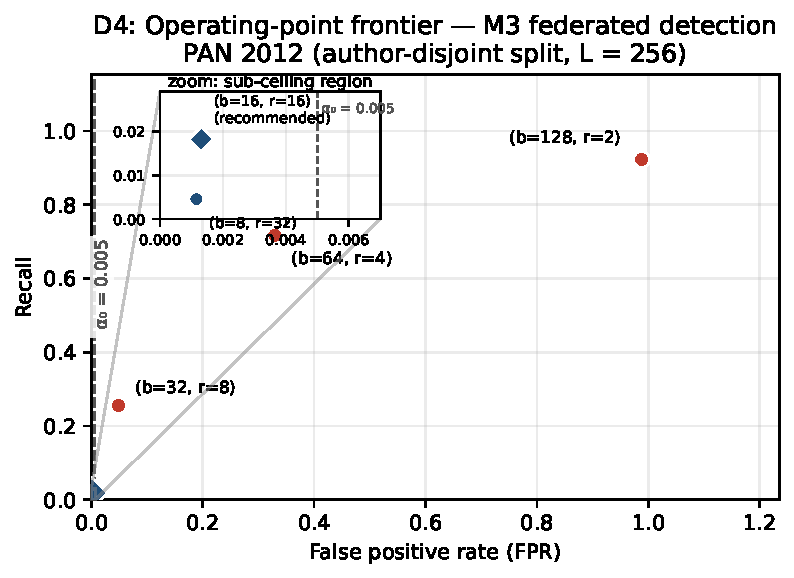
\includegraphics[width=0.78\textwidth]{experiments/results/m3_frontier.pdf}
\caption{The recall/FPR frontier of the signature primitive on real text. Source data: \texttt{m3\_frontier.json}.}
\label{fig:frontier}
\end{figure}

The mechanism of failure is visible in the Jaccard statistics: real conversations executing related adversarial behavior simply do not share enough surface structure. Inter-conversation Jaccard similarity on real text sits far below the $(16,16)$ inflection $J^\star \approx 0.841$, so the S-curve --- which behaves exactly as designed (Sec.~\ref{sec:synthetic}) --- is being evaluated in a region where it correctly returns ``no match.'' The primitive is not broken; the design's assumption about where real adversarial Jaccard mass lies is falsified. Any successor design must either change the representation until related-but-distinct adversarial conversations actually land above the inflection, or abandon set-similarity matching for this layer.

\subsection{RQ3: Does the trajectory model beat the per-message baseline on clean data?}
\label{sec:rq3}

No. The sequence model reaches AUC 0.977 against the baseline's 0.986, and its F1 at the FPR $\leq 0.05$ operating point is lower: the F1 lift is $-0.023$ with bootstrap 95\% CI $[-0.042, -0.002]$ (Table~\ref{tab:clean}) --- the interval lies below zero. On clean data, adding order information through this representation costs performance.

The scope of this negative result should be stated precisely: it falsifies \emph{this} position-weighted sequence representation as a clean-data improvement over a strong per-message baseline on PAN 2012. It does not falsify trajectory modeling in general; richer sequence architectures were not tested. One structural property does survive: the baseline is order-invariant by construction, while the sequence model loses about one point of recall (0.933 $\to$ 0.923) when message order is adversarially shuffled --- and an adversary who destroys conversational order to evade a sequence model also destroys the escalation structure the attack requires. That asymmetry, not clean-data lift, is what the perturbation sweep then probes.

\subsection{RQ4: Does trajectory structure degrade more gracefully under perturbation?}
\label{sec:rq4}

The robustness is real and survives stricter testing; its attribution to trajectory structure does not. We report the original sweep first, then the author-disjoint replication, then the aggregation/order controls that change the interpretation. Table~\ref{tab:sweep} and Figure~\ref{fig:sweep} report the original sweep: both models trained on clean data, thresholds frozen, test positives perturbed with discourse noise at three strengths, five seeds each. The baseline's AUC falls 0.986 $\to$ 0.971 $\to$ 0.949 $\to$ 0.912; the sequence model's falls 0.977 $\to$ 0.968 $\to$ 0.955 $\to$ 0.940. The sequence model's mean AUC drop is smaller at \emph{every} non-zero strength (heavy: 0.037 vs.\ 0.075, roughly half), and the ordering of the two models inverts between medium and heavy noise: the model that loses on clean data wins under perturbation. This is consistent with the earlier single-point observation that a perturbed realism set collapsed the per-message signal (AUC 0.92 $\to$ 0.79 under discourse noise; to 0.13 on an NCMEC-prior-constrained set, where the sequence model retained 0.57) --- but the sweep, unlike those single points, gives a dose-response curve with seed variance.

\begin{table}[!htbp]
\centering
\footnotesize
% Numbers generated from experiments/results/perturbation_sweep.json
% Auto-generated by scripts/build_paper_tables.py
% Source of truth: experiments/results/perturbation_sweep.json
% Do not edit by hand; re-run the script instead.
\begin{tabular}{@{}l c c c c c@{}}
\toprule
 & & \multicolumn{2}{c}{Per-message baseline} & \multicolumn{2}{c}{Sequence model} \\
\cmidrule(lr){3-4}\cmidrule(lr){5-6}
Strength & $p$ & AUC & Drop & AUC & Drop \\
\midrule
none & 0.00 & 0.986 & 0.000 & 0.977 & 0.000 \\
light & 0.15 & 0.971 $\pm$ 0.005 & 0.016 & 0.968 $\pm$ 0.003 & 0.010 \\
medium & 0.35 & 0.949 $\pm$ 0.004 & 0.037 & 0.955 $\pm$ 0.003 & 0.022 \\
heavy & 0.60 & 0.912 $\pm$ 0.010 & 0.075 & 0.940 $\pm$ 0.006 & 0.037 \\
\bottomrule
\end{tabular}

\caption{Perturbation sweep on PAN 2012 (stratified conversation-level split; 5 seeds per non-zero strength; mean AUC $\pm$ across-seed std; drop is relative to the clean condition). Discourse-noise family: truncation, benign-message swap, message drop, order jitter, applied to test positives only. Source: \texttt{perturbation\_sweep.json}.}
\label{tab:sweep}
\end{table}

\begin{figure}[!htbp]
\centering
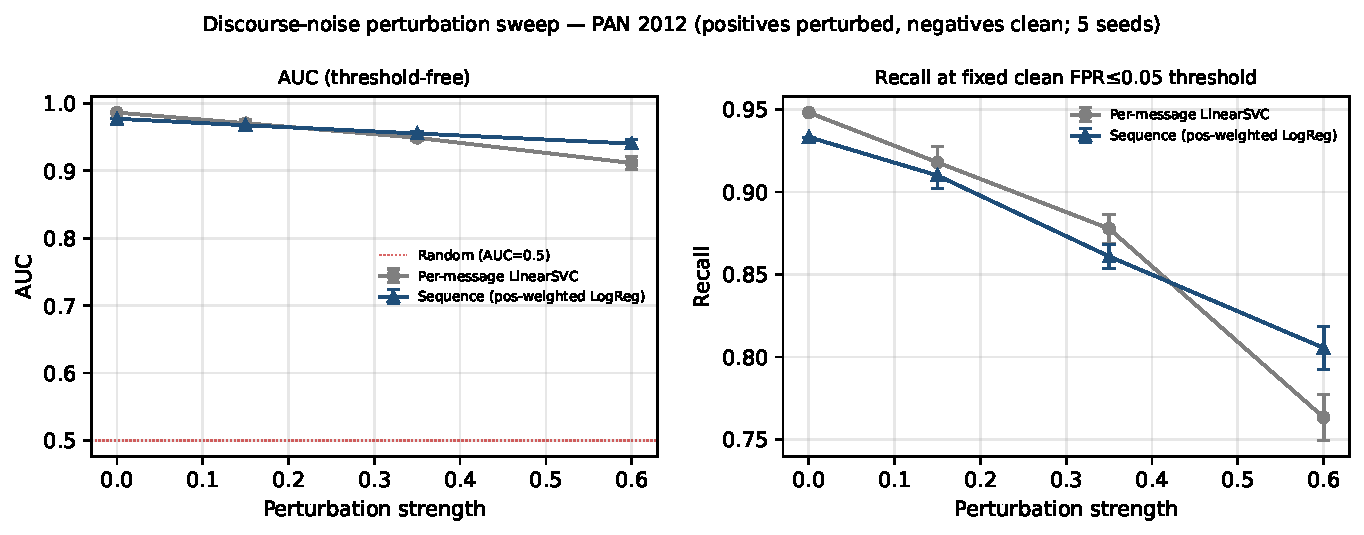
\includegraphics[width=0.9\textwidth]{experiments/results/perturbation_sweep.pdf}
\caption{Degradation of the per-message baseline vs.\ the sequence model across perturbation strengths. Source data: \texttt{perturbation\_sweep.json}.}
\label{fig:sweep}
\end{figure}

\paragraph{The result replicates under the author-disjoint split.}
Table~\ref{tab:sweep-adj} repeats the sweep with no predator author shared between train and test. Clean AUCs compress (baseline 0.975, sequence 0.971), and the ordering under perturbation is unchanged: the sequence model's AUC drop is smaller at every strength, roughly half the baseline's at heavy noise (0.029 vs.\ 0.058). The original result was not an artifact of author leakage across the conversation-level split.

\begin{table}[!htbp]
\centering
\footnotesize
% Numbers generated from experiments/results/perturbation_sweep_author_disjoint.json
% Auto-generated by scripts/build_paper_tables.py
% Source of truth: experiments/results/perturbation_sweep_author_disjoint.json
% Do not edit by hand; re-run the script instead.
\begin{tabular}{@{}l c c c c c@{}}
\toprule
 & & \multicolumn{2}{c}{Per-message baseline} & \multicolumn{2}{c}{Sequence model} \\
\cmidrule(lr){3-4}\cmidrule(lr){5-6}
Strength & $p$ & AUC & Drop & AUC & Drop \\
\midrule
none & 0.00 & 0.975 & 0.000 & 0.971 & 0.000 \\
light & 0.15 & 0.963 $\pm$ 0.010 & 0.012 & 0.964 $\pm$ 0.007 & 0.006 \\
medium & 0.35 & 0.947 $\pm$ 0.007 & 0.028 & 0.958 $\pm$ 0.007 & 0.013 \\
heavy & 0.60 & 0.917 $\pm$ 0.008 & 0.058 & 0.941 $\pm$ 0.007 & 0.029 \\
\bottomrule
\end{tabular}

\caption{Author-disjoint replication of the perturbation sweep (5 seeds per non-zero strength; mean AUC $\pm$ across-seed std). Source: \texttt{perturbation\_sweep\_author\_disjoint.json}.}
\label{tab:sweep-adj}
\end{table}

\paragraph{But matched controls change the attribution: it is aggregation, not order.}
Table~\ref{tab:controls} evaluates seven models/controls on the same author-disjoint split, perturbed conversations, and seeds, and Table~\ref{tab:paired} gives paired bootstrap CIs on the AUC-drop differences. Two facts emerge. First, the sequence model's advantage is real and statistically resolved against every per-message comparison --- mean, max, and top-5 aggregation of message scores, and the concatenation classifier --- with all CIs excluding zero in its favor (the concatenation classifier is the best clean model at AUC 0.989 but degrades \emph{worst} at heavy noise, 0.087). Second, the order-invariant conversation-mean control --- identical to the sequence model except that position weights are removed --- degrades \emph{less} than the sequence model at every strength, with the paired CI excluding zero in the control's favor (heavy: $+0.004$, CI $[+0.002, +0.006]$), and the shuffled-order control tracks the sequence model almost exactly (heavy drop 0.030 vs.\ 0.029). The tested sequence model, in other words, barely uses order at all, and what order sensitivity its position weights add costs a small amount of robustness rather than buying any.

\begin{table}[!htbp]
\centering
\footnotesize
% Numbers generated from experiments/results/perturbation_model_controls.json
% Auto-generated by scripts/build_paper_tables.py
% Source of truth: experiments/results/perturbation_model_controls.json
% Do not edit by hand; re-run the script instead.
\begin{tabular}{@{}l c c c c@{}}
\toprule
 & Clean & \multicolumn{3}{c}{AUC drop at strength} \\
\cmidrule(lr){3-5}
Model / control & AUC & light & medium & heavy \\
\midrule
Per-message mean (baseline) & 0.975 & 0.012 & 0.028 & 0.058 \\
Per-message max & 0.895 & 0.008 & 0.016 & 0.036 \\
Per-message top-5 mean & 0.934 & 0.011 & 0.026 & 0.051 \\
Conversation concat (order-inv.) & 0.989 & 0.010 & 0.024 & 0.087 \\
Conversation mean (order-inv.) & 0.968 & 0.005 & 0.010 & 0.026 \\
\textbf{Sequence (position-weighted)} & 0.971 & 0.006 & 0.013 & 0.029 \\
Sequence, shuffled order (control) & 0.972 & 0.006 & 0.012 & 0.030 \\
\bottomrule
\end{tabular}

\caption{Aggregation and order controls (author-disjoint split, discourse noise, 5 seeds). Clean AUC and mean AUC drop per strength. The conversation-mean control is the sequence model without position weights. Source: \texttt{perturbation\_model\_controls.json}.}
\label{tab:controls}
\end{table}

\begin{table}[!htbp]
\centering
\scriptsize
% Numbers generated from experiments/results/perturbation_paired_tests.json
% Auto-generated by scripts/build_paper_tables.py
% Source of truth: experiments/results/perturbation_paired_tests.json
% Do not edit by hand; re-run the script instead.
\begin{tabular}{@{}l c c c@{}}
\toprule
Comparison & light & medium & heavy \\
\midrule
vs.\ per-message mean (baseline) & $[-0.0202, -0.0054]$$^*$ & $[-0.0239, -0.0080]$$^*$ & $[-0.0365, -0.0165]$$^*$ \\
vs.\ per-message max & $[-0.0217, -0.0052]$$^*$ & $[-0.0198, -0.0043]$$^*$ & $[-0.0471, -0.0193]$$^*$ \\
vs.\ per-message top-5 mean & $[-0.0213, -0.0073]$$^*$ & $[-0.0290, -0.0141]$$^*$ & $[-0.0483, -0.0263]$$^*$ \\
vs.\ conversation concat (order-inv.) & $[-0.0138, -0.0036]$$^*$ & $[-0.0217, -0.0083]$$^*$ & $[-0.0657, -0.0448]$$^*$ \\
vs.\ conversation mean (order-inv.) & $[+0.0004, +0.0034]$$^*$ & $[+0.0007, +0.0050]$$^*$ & $[+0.0018, +0.0064]$$^*$ \\
\bottomrule
\end{tabular}

\caption{Paired stratified bootstrap ($B{=}1000$) 95\% CIs for (sequence AUC drop $-$ comparator AUC drop); negative favors the sequence model; $^*$ marks CIs excluding zero. Source: \texttt{perturbation\_paired\_tests.json}.}
\label{tab:paired}
\end{table}

\paragraph{A second, surface-rewrite perturbation family does not discriminate.}
Under the rule-based surface-rewrite/segmentation family (register substitutions, casing/punctuation jitter, message split/merge), every model is essentially unaffected: the largest mean AUC drop for any model at any strength is under 0.002 (\texttt{perturbation\_second\_family.json}). Character 3--5-gram features are simply insensitive to this rewriting, which is mild good news for all the detectors but means this family provides no evidence either way on the robustness ordering; the aggregation-vs-order attribution rests on the discourse-noise family.

\paragraph{What RQ4 now supports.}
The revised claim is narrower and differently aimed than the design's trajectory hypothesis: \emph{conversation-level averaging --- training and scoring on features averaged over the whole conversation --- degrades roughly half as fast as per-message scoring under discourse noise, on both splits, with paired statistical support; the position/order information in the tested sequence model contributes nothing to that robustness.} The families remain rule-based rather than adaptive, paraphrase/LLM-rewrite attacks are untested, and a genuinely order-sensitive sequence architecture remains unevaluated --- the trajectory hypothesis proper is still open, but it no longer has support from this data.

\subsection{RQ5: Do structurally similar benign conversations absorb disproportionate false positives?}
\label{sec:rq5}

Not on this proxy --- the effect runs the other way. Benign conversations that surface-resemble grooming transcripts (age talk, meeting plans, secrecy language, romantic language) are the population a deployed detector would most plausibly harm: peer support, LGBTQ+ youth conversations, harm-reduction discussion, ordinary adolescent relationship talk. Table~\ref{tab:fps} compares false-positive rates on 500 keyword-matched benign conversations against 500 random benign controls (3 seeds, author-disjoint test negatives). The classifier's FPR on the structurally similar set is \textbf{0.030} against \textbf{0.055} on random controls --- lower, consistently across all three seeds. The MinHash primitive flags almost nothing in either set (0 and 1 conversations total, respectively), as its RQ2 behavior predicts.

\begin{table}[!htbp]
\centering
\footnotesize
% Numbers generated from experiments/results/fp_substrate.json
% Auto-generated by scripts/build_paper_tables.py
% Source of truth: experiments/results/fp_substrate.json
% Do not edit by hand; re-run the script instead.
\begin{tabular}{@{}l c c@{}}
\toprule
Detector & \makecell{Structurally similar benign \\ FPR [pooled Wilson 95\% CI]} & \makecell{Random benign control \\ FPR [pooled Wilson 95\% CI]} \\
\midrule
MinHash $(b{=}16, r{=}16)$ & 0.000 [0.000,\,0.003] & 0.001 [0.000,\,0.004] \\
LinearSVC @ FPR$\leq$0.05 & 0.030 [0.022,\,0.040] & 0.055 [0.045,\,0.068] \\
\bottomrule
\end{tabular}

\caption{False-positive substrate analysis (author-disjoint split; $n=500$ per set; 3 sampling seeds; mean FPR with pooled Wilson 95\% CIs). Keyword filters select for surface similarity to grooming transcripts and are a sampling device, not a classifier. Source: \texttt{fp\_substrate.json}.}
\label{tab:fps}
\end{table}

\begin{figure}[!htbp]
\centering
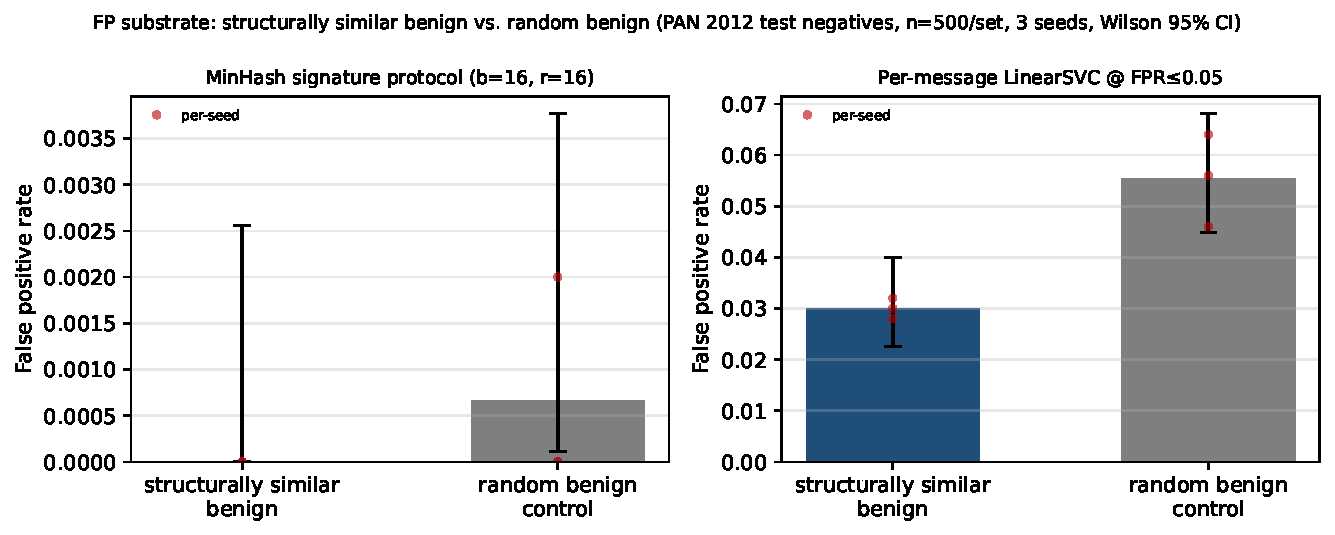
\includegraphics[width=0.85\textwidth]{experiments/results/fp_substrate.pdf}
\caption{FPR on structurally similar benign conversations vs.\ random benign controls, per detector, with per-seed points. Source data: \texttt{fp\_substrate.json}.}
\label{fig:fps}
\end{figure}

Interpretation requires care in both directions. The result weakens the simplistic assumption that surface-similar benign conversations are automatically higher-risk under a lexical detector --- on this substrate they are not, possibly because keyword-matched negatives resemble the classifier's own training negatives. It does \emph{not} clear the deployment concern: PAN negatives are 2012 chat conversations standing proxy for populations the corpus cannot label, and an external sensitive-population substrate (with appropriate ethics review) would be far more probative. What the analysis does establish is the method: substrate-conditional FPR measurement with controls is cheap, and any deployment claim would need it on real substrates.

\subsection{RQ6: What do the simulation and analytical components show?}
\label{sec:rq6}

These results validate mechanisms under stated parameters. They are not deployment evidence and must not be aggregated with the real-data findings above.

\paragraph{Byzantine tolerance (simulation).}
Under the simulated reputation-weighted aggregation, network detection quality degrades less than 5\% up to an empirical Byzantine fraction $\beta^\star = 0.5$ for obvious mis-emitters, and $\beta^\star = 0.4$ against a stealth adversary (\texttt{m8\_byzantine.json}, \texttt{m8\_sprt.json}).

\paragraph{SPRT vs.\ Hoeffding isolation (simulation, weak comparator).}
The sequential test isolates mis-emitting senders about $2.27\times$ faster (mean isolation step) than the EMA-plus-Hoeffding baseline, with SPRT false-isolation rates $\leq 0.044$. The comparison needs a caveat the result file carries as a methodology note: the Hoeffding baseline's own false-isolation rate is extreme ($\approx 0.996$) because it re-applies a fixed-$n$-derived threshold to a high-variance EMA at every timestep with no exoneration state --- an expected consequence of the baseline's definition, not a bug in the SPRT results. The speed comparison on truly misbehaving senders is meaningful; the false-isolation gap should not be quoted as a finding, because the comparator is weak on that axis.

% TODO(bib): [11] (GT-HarmBench, arXiv:2602.12316) is load-bearing for this
% subsection; verify the arXiv ID and author list against the published record
% before submission.
\paragraph{F3 reciprocity (analytical).}
Applying the design's payoff-perturbation mechanism to GT-Harm\-Bench $2\times2$ matrices raises equilibrium cooperation by 0.184 overall and cuts Prisoner's Dilemma defection from 1.0 to 0.57 (\texttt{f3\_reciprocity.json}). This is mechanism design on game matrices. It says nothing about LLM behavior, provider behavior, or deployment.

% =====================================================================
\section{Discussion}
\label{sec:discussion}

\subsection{What the decomposition means for the design}
The design under test bundled three bets: (i) behavioral structure in adversarial conversations is detectable; (ii) that structure can be shared across providers as approximate set-similarity signatures; (iii) trajectory-level modeling is the robust layer. The evidence splits them cleanly. Bet (i) holds on clean historical data (RQ1). Bet (ii) fails on real text (RQ2) --- and it fails at the representation level, not the primitive level, which redirects rather than ends the line of work: the open problem is a manifest representation under which related-but-distinct adversarial conversations achieve high Jaccard while benign traffic does not, and Section~\ref{sec:rq5} shows benign structural look-alikes are not automatically the binding constraint. Bet (iii) fails in the form the design stated it: no clean-data lift (RQ3), and the robustness advantage that initially appeared to support it is attributable, under matched controls, to conversation-level averaging rather than to order information --- the order-invariant twin of the sequence model is at least as robust, and the shuffled-order control shows the tested model barely uses order (RQ4). What survives is a smaller, differently-aimed finding that is still useful to a detection engineer: train and score at the conversation level over averaged features and the detector degrades roughly half as fast under discourse noise as per-message scoring, robustly across splits and with paired statistical support. Whether a genuinely order-sensitive architecture can add robustness \emph{beyond} that aggregation effect is exactly the question this study's simple sequence model cannot answer, and it is now the precise, testable form of the trajectory hypothesis.

\subsection{Failure modes and the false-positive frame}
\label{sec:failure}
The design document cataloged failure modes F1--F7 for a deployed federation; we retain the catalog in compressed form because two of its entries motivated experiments in this paper, and because Appendix~\ref{app:manifest} references it. F1 (signature pollution by a miscalibrated or strategic sender, the A3 case) motivated the M8 simulations: trust-decay scheduling with per-sender precision tracking, where the Hoeffding-derived isolation threshold $\epsilon^\star = \sqrt{\ln(1/\delta)/2n}$ ($\approx 0.083$ at $\delta = 10^{-3}$, $n = 500$) is the design's proposed rule. The RQ6 methodology note adds a caveat the design missed: applied repeatedly to a high-variance EMA rather than a fixed-$n$ average, that threshold false-isolates almost every honest sender --- the IID fixed-$n$ assumption behind the bound does not hold in the sequential setting, and any deployment of the rule would need sequential correction (which is what the SPRT variant is). F2 (false-positive cascade) motivated per-class FP ceilings and the RQ5 substrate method. F3 (free-riding) motivated the analytical reciprocity mechanism, evaluated only on game matrices [11, 14]. F4--F7 (scope creep, signature replay, dictionary attack, trust-root failure) remain design mitigations --- TTLs, rate limits, the minimum-entropy gate $H(\mathbf{f}) \geq H_{\min}$, multi-root PKI --- none of which is validated here.

The overarching frame the false-positive results enforce: at PAN's class balance, even the strong RQ1 classifier yields precision 0.41 at 5\% FPR, so most alerts are false. Any system built on these primitives is a \emph{review-queue prioritizer}, not an enforcement trigger. The design's rule that a match enqueues independent human investigation (Sec.~\ref{sec:decision}) is the minimum viable posture, not a conservatism to be relaxed.

\subsection{Limitations}
\label{sec:limitations}
(1) \emph{Corpus vintage and adversary mismatch.} PAN 2012 records human grooming in 2012-era chat. Every real-data claim is a claim about that distribution; transfer to 2026 platforms, languages beyond English, and hypothesized agentic (A2) operations is untested. (2) \emph{Rule-based perturbation families only.} The robustness ordering is established under the discourse-noise family; the second, surface-rewrite family left every model essentially unaffected and is therefore uninformative for the comparison. Paraphrase/LLM-rewrite families and genuinely adaptive attacks against the deployed detector are untested and could reverse the ordering. (3) \emph{Split coverage.} The RQ4 robustness result now replicates under the author-disjoint split, but the clean-data RQ1/RQ3 numbers are still reported on the conversation-level split and may be optimistic to the extent author style leaks across it (the author-disjoint clean AUCs are lower: 0.975/0.971). (4) \emph{Weak sequence model, now with a measured consequence.} The tested trajectory representation barely uses order (shuffled-order control tracks it; its position weights slightly \emph{hurt} robustness), so RQ4's attribution finding is about this model class; a genuinely order-sensitive encoder remains unevaluated in both directions. (5) \emph{Proxy substrate.} RQ5's benign substrate is keyword-selected PAN negatives, not the real sensitive populations of concern, and the seeds resample overlapping pools. (6) \emph{Simulation and analytical parameters.} M8 and F3 results hold under their stated parameters only.

% =====================================================================
\section{Ethics, Safety, and Governance Non-Claims}
\label{sec:ethics}

\paragraph{Data handling.}
All real-data experiments use the PAN 2012 Sexual Predator Identification corpus, which is public, open research data distributed by the PAN organizers --- and also sensitive online-safety material involving real victims and offenders. The artifact does not redistribute the corpus; provenance and access terms are documented in the repository. No raw dialogue from the corpus appears in this paper, in the artifact's documentation, or in any committed result file: all reported quantities are aggregate metrics, structural labels, and counts. No abuse content, grooming scripts, or operational evasion material was generated in the course of this work; the perturbation families are generic discourse noise (truncation, benign-message dilution, drop, order jitter), not offender tradecraft.

\paragraph{No client-side scanning; no encrypted content.}
Neither the design under test nor this evaluation involves scanning end-to-end encrypted content or client devices. Everything operates over data a platform can already observe under its own policies (Sec.~\ref{sec:oos}).

\paragraph{No deployment recommendation.}
This paper does not recommend deploying the evaluated design or any component of it. The evidence would not support such a recommendation: the signature primitive fails on real data (Sec.~\ref{sec:rq2}), and the one positive robustness signal spans a single perturbation family. The design document's latency, throughput, and topology targets (sub-50\,ms inline matching by analogy to PhotoDNA-class systems [18], 60\,s cache freshness, volumetric extrapolations) are design assumptions from production analogues; no implementation was built or measured here, and none of those numbers is a claim of this paper.

\paragraph{False-positive harms are the central deployment risk.}
Behavioral detectors in this space threaten specific benign populations whose conversations share surface structure with abuse transcripts: minors discussing age and relationships, LGBTQ+ youth seeking support, mental-health peer support, harm-reduction discussion, journalism, and legitimate research. Section~\ref{sec:rq5} measures a proxy for this risk and does not find elevated FPR on PAN keyword-matched negatives --- but that proxy cannot label the real populations of concern, and nothing in this paper clears the risk. Any future deployment-oriented study would need substrate-conditional false-positive measurement on real sensitive-population data, under ethics review, before any operational use.

\paragraph{Human review, appeal, and no automated enforcement.}
A signature or classifier match must never trigger enforcement automatically. The design's own rule --- a match enqueues an independent human investigation (Sec.~\ref{sec:decision}) --- is the minimum posture, and fully automated enforcement would additionally be in tension with GDPR Article~22. Any future system would require an accessible appeals path for affected users and multi-stakeholder scope governance with civil-society representation, on the model of Lantern's externally reviewed governance [17].

\paragraph{No compliance claims.}
This work does not establish compliance with the EU AI Act, GDPR, the UK Online Safety Act, or any other regime; conformity assessment is participant-level work that cannot be done in the abstract [6, 7]. The v8.1 design document's compliance mapping is superseded by this section's non-claims.

% =====================================================================
\section{Research Agenda}
\label{sec:agenda}

The agenda is empirical; nothing here is a deployment step.

\begin{itemize}[leftmargin=1.5em]
\item \textbf{Genuinely order-sensitive sequence models.} Now the top item: RQ4's controls show the tested sequence model derives its robustness from averaging, not order. The precise open question is whether a phase-transition model or structured sequence encoder can add robustness \emph{beyond} the conversation-mean control, under the same sweep and paired-test framework --- that comparison, not a baseline comparison, is the test the trajectory hypothesis now requires.
\item \textbf{Paraphrase / LLM-rewrite perturbation family.} The rule-based surface-rewrite family left character n-gram models unaffected; a semantic rewrite family (run locally, without sending corpus text to external APIs) is the remaining untested attack on the lexical features all these models share.
\item \textbf{External benign substrates.} Substrate-conditional FPR measurement on real sensitive-population data (peer support, harm reduction, adolescent relationship conversations), under ethics review, to replace the RQ5 proxy.
\item \textbf{Manifest representations beyond MinHash.} RQ2 falsifies set-similarity matching over the current manifest, not cross-provider matching per se. Candidate directions: learned embeddings with calibrated similarity thresholds, class-level (rather than content-shingle) manifests with measured real-data Jaccard distributions, or exchange of classifier scores rather than signatures.
\item \textbf{Formal privacy and false-positive analysis.} The unlinkability (SG2) and minimization (SG4) properties are asserted at schema level; a formal analysis, and a false-positive cost model that includes substrate-conditional harm, are both open.
\item \textbf{Deployment, last.} Only after substantial validation on the above --- including adaptive-adversary evaluation --- would pilot deployment of any component be defensible.
\end{itemize}

% =====================================================================
\section*{References}
\addcontentsline{toc}{section}{References}
\small
\emergencystretch=1.5em % tolerate slightly looser lines rather than overfull arXiv IDs
\begin{enumerate}[label={[\arabic*]}, leftmargin=2.4em, itemsep=2pt]
\item[{[1]}] Prompt Injection Attacks on Agentic Coding Assistants: A Systematic Analysis of Vulnerabilities in Skills, Tools, and Protocol Ecosystems. SoK, arXiv:2601.17548, January 2026.
\item[{[2]}] Are AI-assisted Development Tools Immune to Prompt Injection? Empirical evaluation of seven major MCP clients (Claude Desktop, Claude Code, Cursor, Cline, Continue, Gemini CLI, Langflow). arXiv:2603.21642, March 2026.
\item[{[3]}] Anthropic MCP Design Vulnerability Enables RCE, Threatening AI Supply Chain. Disclosure of CVE-2025-49596 (MCP Inspector), CVE-2026-22252 (LibreChat), CVE-2026-22688 (WeKnora). The Hacker News, April 2026.
\item[{[3a]}] EchoLeak: The First Real-World Zero-Click Prompt Injection Exploit in a Production LLM System. CVE-2025-32711 (CVSS 9.3); Aim Labs disclosure and Microsoft MSRC patch, June 2025; technical writeup arXiv:2509.10540.
\item[{[4]}] Breaking the Protocol: Security Analysis of the Model Context Protocol Specification and Prompt Injection Vulnerabilities in Tool-Integrated LLM Agents. arXiv:2601.17549.
\item[{[5]}] The Tech Coalition. 2025 Annual Transparency Report and Lantern Transparency Report; Initiate 2026 hackathon proceedings (VHIP, Korean grooming classifier). April 28, 2026.
\item[{[6]}] European Commission. Guidelines for Providers of General-Purpose AI Models; EU AI Act Implementation Timeline (enforcement effective 2 August 2026).
\item[{[7]}] European Commission. General-Purpose AI Code of Practice, Safety and Security Chapter, Measure 5.1 (agentic capabilities and autonomous use).
\item[{[8]}] Maiya, S., Bartsch, H., Lambert, N., \& Hubinger, E. Open Character Training: Shaping the Persona of AI Assistants through Constitutional AI. arXiv:2511.01689.
\item[{[9]}] Tan, D., Woodruff, A., Warncke, N., Jose, A., Rich\'e, M., Africa, D.~D., \& Taylor, M. Inoculation Prompting: Eliciting traits from LLMs during training can suppress them at test-time. arXiv:2510.04340, 2025. (Attribution corrected against the arXiv record, 2026-07-07.)
\item[{[10]}] Geddes et al. Red-Teaming Medical AI: Systematic Adversarial Evaluation of LLM Safety Guardrails in Clinical Contexts. medRxiv preprint 10.64898/2026.02.26.26347212v1, 2026. (Preprint; LLM-as-judge harm scoring; physician review pending.)
\item[{[11]}] Cobben et al. GT-HarmBench: Benchmarking AI Safety Risks Through the Lens of Game Theory. arXiv:2602.12316, 2026.
\item[{[12]}] Villatoro-Tello, E., Ju\'arez-Gonz\'alez, A., Escalante, H.~J., Montes-y-G\'omez, M., \& Villase\~nor-Pineda, L. A two-step approach for effective detection of misbehaving users in chats. PAN 2012 Sexual Predator Identification shared task at CLEF, 2012.
\item[{[13]}] Greshake, K., Abdelnabi, S., Mishra, S., Endres, C., Holz, T., \& Fritz, M. Not what you've signed up for: Compromising Real-World LLM-Integrated Applications with Indirect Prompt Injection. arXiv:2302.12173, 2023.
\item[{[14]}] Ostrom, E. Governing the Commons: The Evolution of Institutions for Collective Action. Cambridge University Press, 1990.
\item[{[15]}] Broder, A.~Z. On the resemblance and containment of documents. Proceedings of Compression and Complexity of Sequences (SEQUENCES '97), 1997.
\item[{[16]}] Peters, G., et al. Deep Fake Frauds: When You Lose Trust in Your Own Ears and Eyes. Alliance to Counter Crime Online (ACCO), 2024.
\item[{[17]}] BSR (Business for Social Responsibility). Human Rights Impact Assessment of the Tech Coalition's Lantern Program.
\item[{[18]}] Microsoft Corporation. Update to PhotoDNA: sub-millisecond search performance against ten-million-hash databases on x64 and Arm64 hardware. Microsoft Digital Safety, 2023.
\item[{[19]}] Adversarial Intent Telemetry: reproducible artifact. \url{https://github.com/gillfahrawn/adversarial-intent-telemetry}, 2026. Includes result JSONs, claim-consistency checker, table generator, truth ledger, and validity-boundary statement.
\end{enumerate}

\vspace{1em}
\hrule
\vspace{0.5em}
\noindent\small\emph{This is a working draft of an empirical study intended for circulation and review. The v8.1 design document it evaluates is included with the artifact. Substantive technical critique and replication attempts are welcome.}

% =====================================================================
\appendix
\section{Feature Manifest Schema for the Evaluated Design}
\label{app:manifest}

This appendix defines the canonical feature manifest schema of the design under test. It is normative \emph{only} for reproducing or evaluating this design --- it is not proposed as a production standard, and the RQ2 result (Sec.~\ref{sec:rq2}) means the signature layer built on this schema should not be deployed as specified. The schema is retained in full because it makes the evaluated design implementable without reconstruction from prose, and because the manifest vocabulary is a reusable starting point for the representation work in the research agenda.

\paragraph{Schema versioning.} Manifests carry a \texttt{manifest\_version} string of the form \texttt{fm-YYYY-MM} identifying the schema revision. A receiver rejects manifests whose version is not in its \textsc{SupportedManifests} set (Algorithm~\ref{alg:handshake}).

\paragraph{Manifest as a multiset of structural feature tokens.} The manifest is a multiset of typed feature tokens of cardinality $|f| \in [32, 128]$ (the sanity check in Sec.~\ref{sec:synthetic} uses $|f| = 64$). Each token is a \texttt{(field, value)} tuple drawn from the fields below, canonically ordered before hashing (MinHash is order-invariant; ordering matters only for byte-stable attestation).

\renewcommand{\arraystretch}{1.35}
{\footnotesize
\begin{longtable}{@{}p{2.6cm} p{1.6cm} p{2.3cm} p{7.5cm}@{}}
\caption{Feature manifest schema of the evaluated design. $^\dagger$\,enum cardinalities are recommended values. Every field is structural; no field encodes raw prompt text, user identity, or model weights (the design's privacy invariant, Sec.~\ref{sec:decision}).}
\label{tab:manifest-schema} \\
\toprule
\thead{Field name} & \thead{Type} & \thead{Cardinality} & \thead{Source primitive, encoding,\\and entropy contribution} \\
\midrule
\endfirsthead
\multicolumn{4}{l}{\footnotesize\itshape Table~\ref{tab:manifest-schema} (cont.)}\\
\toprule
\thead{Field name} & \thead{Type} & \thead{Cardinality} & \thead{Source primitive, encoding,\\and entropy contribution} \\
\midrule
\endhead
\midrule
\multicolumn{4}{r}{\footnotesize\itshape continued on next page}\\
\endfoot
\bottomrule
\endlastfoot

\texttt{intent\_class} & enum$^\dagger$ & 1--3 tokens & Output of the local classifier stack. One or more of \{\textit{reframe}, \textit{euphem}, \textit{decomp}, \textit{role\_inj}, \textit{hypoth}, \textit{ctx\_poison}\} from Table~\ref{tab:taxonomy}. Encoded as \texttt{(intent\_class, label\_id)}. Entropy contribution: $\log_2 6 \approx 2.58$ bits per token, uniform over 6 classes. \\

\texttt{behavior\_phase} & enum$^\dagger$ & 0--2 tokens & Latent phase label from the trajectory classifier (Sec.~\ref{sec:trajectory}). One of \{\textit{rapport}, \textit{isolation}, \textit{desensitize}, \textit{sexualize}, \textit{coerce}\} for grooming. Encoded as \texttt{(behavior\_phase, label\_id)}. Entropy contribution: $\log_2 5 \approx 2.32$ bits per token. \\

\texttt{phase\_transition} & enum$^\dagger$ & 0--1 token & Detected phase-transition signal in the current window, one of $\{\bot, \mathrm{rapport}{\to}\mathrm{isol}, \mathrm{isol}{\to}\mathrm{desens}, \ldots\}$. Entropy contribution: $\sim 3$ bits per token for grooming's five-state chain. \\

\texttt{embed\_anom\_bin} & ordinal & 8--16 tokens & Embedding-space anomaly score from the local classifier, quantized to $B = 16$ bins. Encoded as \texttt{(embed\_anom\_bin\_$k$, 1)} for each bin $k$ exceeding the participant's calibration threshold. Quantization is the canonicalization step intended to make cross-provider matching tolerant of embedding-stack drift. Entropy contribution: $\log_2 16 = 4$ bits per token. \\

\texttt{role\_marker} & enum$^\dagger$ & 0--6 tokens & Presence flags for role-injection markers, drawn from \{\textit{researcher}, \textit{developer}, \textit{parent}, \textit{law\_enf}, \textit{system\_role}, \textit{red\_team}\}. Entropy contribution: $\log_2 6 \approx 2.58$ bits per token. \\

\texttt{hypoth\_frame} & enum$^\dagger$ & 0--4 tokens & Hypothetical-sandboxing frame markers drawn from \{\textit{fiction}, \textit{simulation}, \textit{training}, \textit{worldbuild}, \textit{academic}\}. Entropy contribution: $\log_2 5 \approx 2.32$ bits per token. \\

\texttt{decomp\_signal} & ordinal & 4--16 tokens & Cross-turn intent-aggregation score from the sequence classifier (Sec.~\ref{sec:trajectory}), quantized to $B = 8$ bins per turn over a sliding window of up to $k = 16$ turns. Encoded as \texttt{(decomp\_signal, turn\_idx, bin)}. Entropy contribution: $\log_2 (8 \cdot 16) = 7$ bits per token. \\

\texttt{prem\_drift} & ordinal & 0--8 tokens & Premise-drift signal: divergence between the structured belief-state at turn $t$ and at turn $t - k$ for $k \in \{1, 2, 4, 8\}$, quantized to $B = 8$ bins. Entropy contribution: $\log_2 (8 \cdot 4) = 5$ bits per token. \\

\texttt{provenance\_fail} & enum$^\dagger$ & 0--3 tokens & Retrieval-channel provenance failure markers (cf.\ the MCP context in Sec.~\ref{sec:mcp}), drawn from \{\textit{instr\_in\_data}, \textit{cross\_tool\_inject}, \textit{unattested\_source}\}. Entropy contribution: $\log_2 3 \approx 1.58$ bits per token. \\

\texttt{demographic\_prior} & enum$^\dagger$ & 0--1 token & Inferred demographic-asymmetry prior (e.g., inferred adult-to-minor interaction), used by the design to raise sensitivity (Sec.~\ref{sec:trajectory}). Non-default priors only. Entropy contribution: $\sim 1$--2 bits per token. \\

\texttt{scope\_class} & enum$^\dagger$ & 1 token & Coarse harm-category gate matching the payload \texttt{scope} field, $\subseteq$ \{\textit{CSAM}, \textit{CSAE}, \textit{sextortion}\}. Low-entropy by design; disambiguates cache lookup. Entropy contribution: $\log_2 3 \approx 1.58$ bits per token. \\

\end{longtable}
}

\paragraph{Minimum-entropy gate.} The aggregate Shannon entropy $H(\mathbf{f})$ is computed from the per-token contributions above, weighted by the empirical token-presence distribution at the emitting participant. The gate $H(\mathbf{f}) \geq H_{\min}$ (Algorithm~\ref{alg:handshake}) is the design's structural defense against dictionary attack (failure mode F6, Sec.~\ref{sec:failure}); the recommended $H_{\min} = 24$ bits was calibrated against per-querier rate limits and signature TTL. The gate and its recommended value are design context; neither is empirically evaluated in this paper.

\paragraph{Canonical serialization.} Before signing, the manifest's source representation is canonicalized to JCS (RFC 8785); the attestation covers the canonical bytes, and the MinHash signature in the wire payload (Listing~\ref{lst:payload}) is computed over the same representation.

\paragraph{Forward compatibility.} The schema is open to extension through new fields, enum values, and quantization choices via the \texttt{manifest\_version} mechanism; receivers reject unsupported versions rather than ingesting unrecognized fields.

\end{document}
